\documentclass{article}
\usepackage{amsmath}
\usepackage{cite}
\usepackage{amssymb}
\usepackage{amsfonts}
\usepackage{graphicx}
\usepackage{textcomp}
\usepackage{xcolor}
\usepackage{subcaption}
\usepackage{float}

\begin{document}

\title{Classificador bayesiano no dataset Parkinson.}

\author{Arthur Felipe Reis Souza \\
Electrical Engineering Department, \\
Federal University of Minas Gerais, \\
Belo Horizonte, Brazil \\
arthurfreisouza@gmail.com \\
\and
Antônio de Pádua Braga and Frederico Gualberto Ferreira Coelho \\
Electrical Engineering Department, \\
Federal University of Minas Gerais, \\
Belo Horizonte, Brazil \\
apbraga@cpdee.ufmg.br, fredgfc@ufmg.br
}

\maketitle

\begin{abstract}
   % Abstract content here.
\end{abstract}

\section{Introdução}

Este relatório tem por objetivo mostrar o processo de classificação bayesiana. As bases de dados que serão a XOR e duas distribuições normais.

\section{Dados}

Os dados foram gerados através de distribuições normais, e estão retratados nas imagens abaixo : 

\begin{figure}[h]
    \centering
    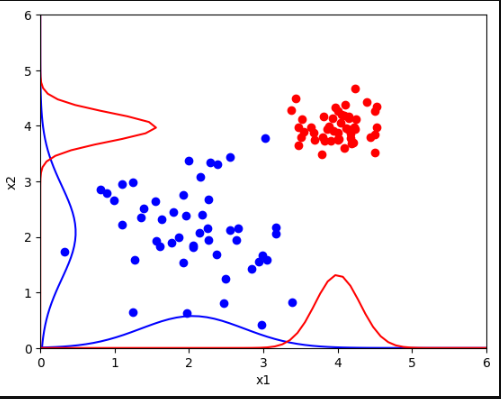
\includegraphics[width=0.75\linewidth]{normal_dit.png}
    \caption{Dados gerados por 4 distribuições normais.}
    \label{fig:kernel_types}
 \end{figure}

 \begin{figure}[h]
    \centering
    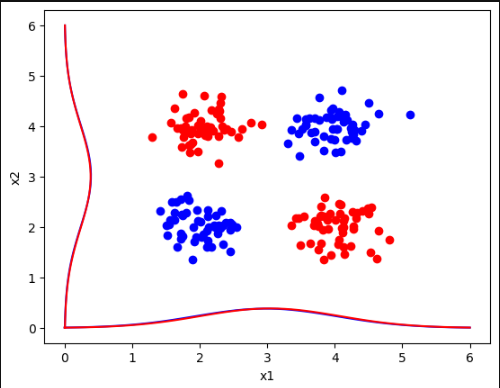
\includegraphics[width=0.75\linewidth]{xor_distribution.png}
    \caption{4 distribuições geradas, seguindo a lógica da XOR.}
    \label{fig:kernel_types}
 \end{figure}



 \section{Aplicação do algoritmo}

 O classificador bayesiano leva em consideração a independência entre os atributos, bem como a probabilidade a priori de ocorrência da classe ao realizar a classificação. Ele se baseia no teorema de Bayes, que é descrito pela seguinte equação:
 
 \[
P(C|X) = \frac{P(X|C) \cdot P(C)}{P(X)}
\]

Apesar de considerar a independência entre as características, o mesmo pode ser extendido para casos onde há uma certa correlação entre os atributos. Nesses casos, o classificador irá considerar a matriz de covariâncias na estimativa da função densidade.

\begin{figure}[h]
    \centering
    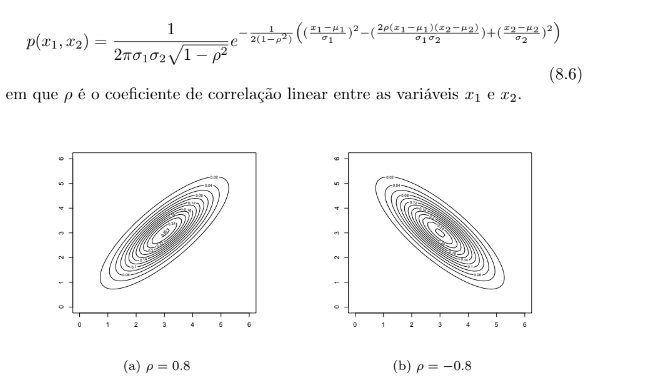
\includegraphics[width=0.75\linewidth]{caso_geral_bayes.png}
    \caption{Equação geral da estimativa do classificador de bayes Multivariado.}
    \label{fig:kernel_types}
 \end{figure}

\section{Resultados}

Após aplicar o classificador bayesiano em ambas as bases de dados e, utilizando o K-Fold Cross Validation, com K = 10, obtemos que a acurácia de 72\%. A superfície de separação para essa base de dados é mostrada abaixo :


\begin{figure}[h]
    \centering
    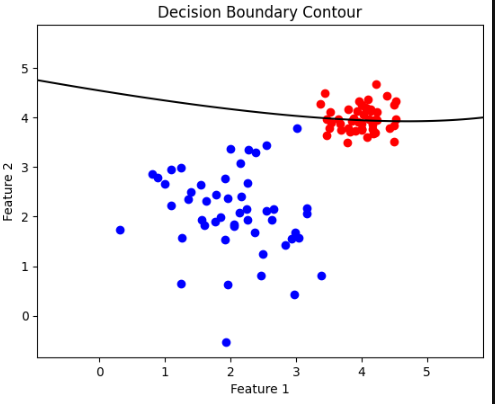
\includegraphics[width=0.75\linewidth]{surface_plot.png}
    \caption{Superfície de separção base de dados 1.}
    \label{fig:kernel_types}
 \end{figure}

Apesar de uma acurácia aceitável, o resultado não foi bom.

\vspace{1cm}

Para a segunda base de dados, a acurácia obtida foi de 81\%.
\section{Conclusão}

Com este relatório, foi possível observar o classificador bayesiano em duas base de dados distintas. Os resultados obtidos mostram que o classificador teve um bom desempenho na base de dados 1, mas melhorou consideravelmente na base de dados 2. A matriz de covariâncias, nesse caso, contribuiu consideravelmente na predição de uma nova amostra.

\end{document}
